%!TEX root = ../main.tex
In this chapter we briefly introduce SME as well as CSP and in more detail, we introduce SMEIL and \cspm along with the FDR4 tool and its cababilities.

\section{Synchronous Message Exchange}
Since SMEIL is based on the SME model, we give a brief introduction to SME to familiarize the reader with the SME model before introducing SMEIL.
\\

The development of SME was mainly driven by the need to provide a simple framework for programming a Field Programmable Gate
Array, FPGA, since FPGAs can achieve the same performance as a General Purpose Graphical Processing Units, GPGPU, but with much less energy consumption. GPGPUs have been extensively researched and different environments have been implemented to give programmers the posibility of utilizing the cababilities of it, but FPGAs are a far better choice when it comes to energy sensitive applications. The FPGA has not been the subject of as much research as the GPGPU, and when using FPGAs, the developer need to design an integrated circuit on the gate level, which is difficult and not common knowledge these days.
Unfortunately designing hardware is often a tedious task but with SME it becomes more accessable to design and implement hardware models.

SMEs main target is to give software developers a tool which provide the opportunity for the developer to program hardware but with a distance from the hardware details, so in a way, the development resembles the structures and semantics that is known from software development.
Thus the framework is based of a top-down approach rather than a bottom-up approach that is common in the current hardware frameworks.
% Global synchronicity is fundamental when modeling hardware, but CSP does not support this. Even though CSP does enforce strict synchrony between communicating processes, there is no such semantic beging enforced on a global level. % TODO: Do I want to include this?

SME was first introduced in 2014 and after several iterations~\cite{Vinter2014, Vinter2015, Skovhede} now presents as a programming model, a simulation library, and VHDL code generators~\cite{vhdl}. The original idea was conceived following an attempt to create hardware descriptions from a vector processor model, modeled in PyCSP~\cite{bjorndalen2007pycsp},
% TODO: Figure out what the correct reference to this is.
a Communicating Sequential Processes (CSP)~\cite{hoare1978communicating} library for Python.\\

The work was initially presented in the paper \textit{BPU Simulator}~\cite{Rehr2013}. This paper only introduced a high abstraction level simulation and therefore the subject was explored more in detail in the master thesis project \textit{Generation of FPGA Hardware
Specifications from PyCSP Networks}~\cite{Skaarup14}. From the results of the master thesis it was clear that PyCSP could be used to model hardware however the need to enforce global synchrony to the circuit resulted in an explosion in the number of channels for controlling the progress and for simulating the clock, and even simple circuits would become overwhelmingly large.\\

The design approach of the master thesis was to implement a clock process that would drive the circuit. This meant that each process must read the clock signal and in order to avoid race conditions the system had to be implemented with a two-way clock, the so called \textit{tick} and \textit{tock} signals. Since deadlocks can happen in CSP it was important to implement deadlock prevention, which was done by adding channels with a single buffer element. This way, no processes would end up in a deadlock. Figure \ref{fig:sme:clock_latch} shows how a simple CSP network would be modelled in the synchronous PyCSP model. It is clear how trying to use PyCSP for modelling synchronous hardware would result in extremely large networks.
\begin{figure}[h!]
\centering
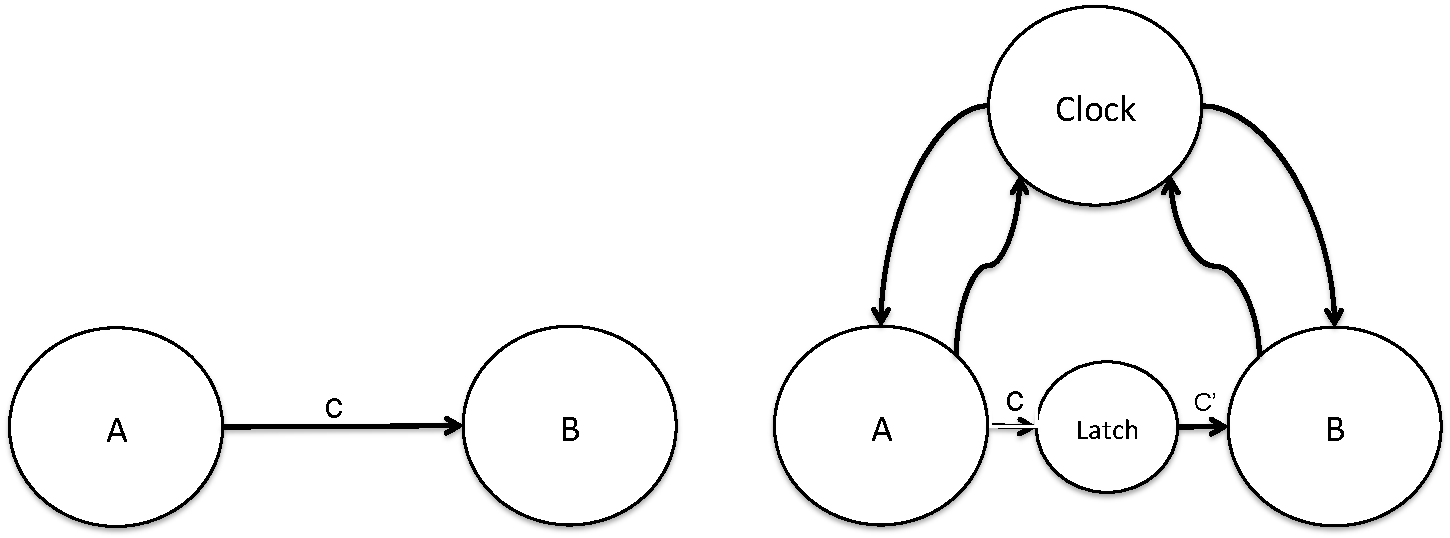
\includegraphics[width=10.0cm]{figures/clocked.pdf}
\caption{To enforce global synchrony on a simple reader-writer network in CSP, the complexity increase to include the clock and latch. Figure from \cite{Vinter2014}}
\label{fig:sme:clock_latch}
\end{figure}
\\\\
The advantage of using Python for this kind of processor simulation is the flexibility and simplicity of the language. It is easy to experiment with various ideas and versions but with the increased complexity of the added clock process and and clock-signal propagation, the advantages of Python seemed to diminish. Therefore the conclusion from the master thesis was that using PyCSP alone for building synchronous processor simulators was not feasible since the global clock was forced onto the CSP model. It was also concluded that external choice, which is a powerful and essential part of CSP, was not utilized in the globally synchronous approach. They did, however, conclude that several of other CSP concepts was fitting well with the hardware concepts, such as shared-nothing in CSP matches the structure of hardware communication.\\

After this attempt, it became clear that the structure of CSP was poorly suited for modeling clocked systems, and therefore it was decided to create the Synchronous Message Exchange framework, based on the CSP algebra. The idea was to only use the subset of the CSP algebra that provided beneficial functionality to hardware modeling which, most importantly, meant that external choice was omitted. However, the shared-nothing property of CSP showed to be very useful, since the network state could only be changed by process communication.
\\
% In SME the introduction of an implicit clock that eliminates the complexity caused by the model, described above, was imperative and is one of the key concepts hereof. The implicit clock removed the problems found by forcing the globally synchronous clock onto the CSP model. \\
In SME, a network is a combination of processes that are connected through buses. The processes communicate through a collection of signals in a bus, instead of CSP's synchronous rendezvous model, but retains the shared-nothing trait of CSP.
SME uses the term \texttt{bus} instead of \texttt{channel} to enforce the semantic correlation between the SME bus and a physical hardware signal bus.
The process communication is handled by a hidden clock which eliminates the complexity that arose from adding synchronicity to a CSP network. The combination of the hidden clock and the synchronous message passing between processes means that the SME model provides hardware-like signal propagation.

An SME clock cycle consists of three phases: it reads, executes, and writes as can be seen in Figure~\ref{fig:sme_process_flow}. The process is activated on the rising clock edge where it reads from the bus and it reads, executes and writes to the bus in one clock cycle. Just before the rising edge of the clock, all signals are propagated on all buses which means, that all communication happens simultaneously. Because of this structure, if a value is written by a process in cycle $i$, it is read by the receiving process in cycle $i+1$.

SME is able to detect read/write conflicts where multiple writes are performed to a single bus within the same clock cycle as well as reads from a signal that has not been written to in the previous clock-cycle.\\
All data, that are written to a bus can be logged for each clock cycle which means that these logs can be saved in a Comma-Separated Values, CSV, format and used for validating the VHDL implementation with a VHDL tool. This would eliminate the need to write seperate VHDL tests which will improve developer productivity immensely.

SME also supports clock-multipliers which means that a clocked network can have components inside the network being clocked at a different rate than its own clock. The rate can be an integer multiplier from its own clock. This means that all components are clocked relative to its parent network and therefore the clock will not need any extra coordination. It does however mean that the inner components can only fun faster than their parents.
% TODO: Do I really want this included?

Since an SME network is a network that can be represented as a graph, a diagram tool have also been implemented for SME. It utilizes the Graphviz tool to generate a visual graph of the network. This means that the SME networks can be generated and drawn as a graph which can help with debugging.
%TODO: Also, it this something I really want to include?


\begin{figure}[!ht]
  \centering
  \begin{tikzpicture}[auto]
    \node[mycircle, text width=2cm, shape=rectangle] (read) {Read};
    \node[mycircle, text width=2cm, shape=rectangle] (execute) [below=0.5cm of read] {Execute};
    \node[mycircle, text width=2cm, shape=rectangle] (write)  [below=0.5cm of execute] {Write};

    \draw [myarrow] (read) -- (execute);
    \draw [myarrow] (execute) -- (write);
    \draw [myarrow] (write) |-([shift={(5mm,-5mm)}]write.south east)-- ([shift={(5mm,5mm)}]read.north east)-| (read);
  \end{tikzpicture}
  \caption{SME process flow for one clock cycle.}
  \label{fig:sme_process_flow}
\end{figure}
Since SME is based on CSP, all SME models have a
corresponding CSP model, and because of this property, we are able to create a transpiler translating SME models to \cspm{}.
The SME model is currently implemented as libraries for the general-purpose languages C\#~\cite{Skovhede}, C++~\cite{asheim2015}, and Python~\cite{asheim2016vhdl}. The Python and C\# libraries both have code generators for VHDL as well.

\subsection{SMEIL}
% TODO: Add more to this section. I have more space in my thesis and SMEIL can easily be explained a bit further.
\label{SMEIL-section}
With the different SME implementations, a need arose for a common intermediate language. SMEIL was developed as a Domain Specific Language (DSL) for SME, usable both as an Intermediate Language, IL, and as an independent implementation language. It has a C-like syntax with a specialized type system that makes hardware modeling simple. In spite of its simplicity, SMEIL still provides hardware-specific functionality that is more difficult to create with general-purpose languages.
Often when modeling hardware in Hardware Description Languages (HDLs) like VHDL or Verilog, code for testing and verifying are often written in the same language as the design itself. Unfortunately, the HDLs often does not have the functionality for generating proper simulation input. Using general-purpose languages for testing hardware models are useful since the range of available libraries are much larger.
Therefore the SMEIL simulator provides a simple language-independent API which enables SME implementations written for general-purpose languages to communicate with SME networks written in SMEIL, so-called co-simulation.


The base entity of an SMEIL program is the module which corresponds to a file. The module consists of the actual SMEIL program as well as information like import statements. SMEIL programs can be seperated into modules which can then be importet into other SMEIL programs, creating a library-like structure and have reusable components. \\
\begin{listing}
\begin{minted}[escapeinside=||, mathescape=true]{smeil_lexer.py:SMEILLexer -x}
proc addone (in inbus)
    bus outbus {
        val: int;
    };
{
    outbus.val = inbus.val + 1;
}

    |$\vdots$|

network net() {
    instance a of addone(b.outbus);
    instance b of ..
    |$\vdots$|
}
\end{minted}
\caption{Small example of process and network syntax in SMEIL.}
\label{lst:smeil_small_syntax_example}
\end{listing}

The two fundamental components of an SMEIL program is \texttt{process} and \texttt{network}. The process consists of variable and bus definitions, as well as the statements that are evaluated once for each clock cycle. The purpose of the \texttt{network} declaration is to define the relations between each entity in the program. A small example of process and network syntax can be seen in Listing~\ref{lst:smeil_small_syntax_example}.

There are several different ways to use SMEIL, one being co-simulation as described above. However, in this work, we focus on the independent SMEIL representation and thus we only present examples in pure SMEIL. These pure SMEIL programs must contain a process which generates input for the network since the network cannot receive input elsewhere. The program is simulated using the command line tool. Simulation is done in order to test the design of the system.

During the simulation, ranges for all observed values are captured so the observed values and types can be used to constrain the original defined types and ranges. This property is of great value when translating into \cspm{}, and when creating assertions, since we can use these values to actually assert the network.
The number of clock cycles, that the simulation is run for, is specified by the programmer via the command line tool. If the simulation is not passing through enough clock cycles, the verification might be inadequate. Since the verification builds on the observed values, the simulation needs to be long enough such that the whole possible range of input values is exhausted.

% ------------------------
% "The purpose of the sync and async modifiers of processes, which are seen in the
% <process> production of the grammar, is to distinguish between processes which are
% run during every clock-cycle and processes which are only run when they receive a
% signal on their input buses. If neither modifier is specified, the process defaults to sync .
% async processes are not supported in the current implementation."



% "SMEIL is a strongly, statically typed language with a simple type system that is checked
% at compile-time. Since hardware is static and SMEIL is targeted towards creating hard-
% ware descriptions, we want a type system which is capable of enforcing as many static
% invariants as possible. This means that no implicit type coercion is performed except
% between signed and unsigned integers. Consequently, there is no implicit notion of
% truthness (i.e., if (1) { results in a type error) and only expressions of boolean type
% can be used in conditionals. These restrictions ensure that SMEIL can be straightfor-
% wardly transformed to a wide range of target languages; it is easy to transform a stati-
% cally typed language to one which is dynamically typed, but not the other way around.
% The primary feature which distinguishes the type systems of SMEIL and general-
% purpose languages is the support for bit-precise types. General-purpose languages tar-
% get CPUs which has fixed-width registers and are typically unable to work with units of data smaller than a byte. When targeting custom hardware, we are free to define wires
% of exactly the width we need. Determining the minimum width of a wire is a prereq-
% uisite for avoiding wasted space leading to a less efficient hardware implementation.
% SMEIL supports integers constrained to a specific bit-length, unlimited-size inte-
% gers, booleans, double and single precision floating point and string. Fixed-length ar-
% rays of these primitive types may also be created. Floating-point numbers are only
% there for completeness but are currently not supported in hardware-translations due to
% the spotty floating-point support in FPGAs (although this situation is improving). The
% naming scheme for types is simple and follows a predictable pattern (the full grammar
% is shown in Figure .). For integer types, the prefixes i and u refers to signed and
% unsigned integers respectively. A prefix is followed by a number determining the bit-
% length of the type. For example, i13 is a -bit signed integer. Unlimited-size integers
% are also supported (more on those in Section .) and are denoted simply as int and
% uint . Finally, bool , f32 and f64 denotes booleans and single- and double-precision
% integers respectively. Array types are created by prefixing a type with a number of ele-
% ments. For example, [10]i4 denotes an array of  -bit signed integers.
% The type checker of libsme determines the validity of types in a SMEIL program
% through a number of simple type unification rules (Table .). For all non-integer
% types, the rules are simple: only truly identical types unify. For integer types with a
% constrained bit-length, the following rules apply: Two integer types with different bit-
% lengths are unified to the largest. Two types of different signedness are unified to a signed integer with a size taking the sign-bit into account. The reasoning behind this
% is the following: when unifying a signed and an unsigned number, the resulting type
% should be able to hold the largest number representable by either of the two types. For
% example, if we unify the types u8 and i8 , the result is i9 instead of i8 . Otherwise,
% if the unsigned number was larger than 2 7 the type conversion itself would cause an
% overflow. Also, as seen from the table, the lengths of arrays are not taken into account
% as this would be overly restrictive. For instance, the expression a[3] + b[2] would
% be invalid if a and b were arrays of different lengths.
% Types are enforced on assignment meaning that the following declarations are in-
% valid:
% const foo: i32 = 3;
% var bar: u16 = foo;
% since they assign foo , a -bit signed integer constant, to bar a -bit signed integer
% variable. However, the following declarations
% const foo: i32 = 3;
% var bar: uint = foo;
% are valid since i32 and uint unifies to i32 .
% We realize that this model has several limitations. In particular, unifying two dif-
% ferently sized types to the largest does not ensure that the result of a binary operation
% on two values will not overflow the destination type. On the other hand, unifying types
% to sizes large enough that the result can not overflow often leads to a significant over-
% estimation of required bit-widths. Likewise, binary operators which may produce a
% result smaller than either of its operands are not taken into account. The currently im-
% plemented type checker also does not consider the constness of values, which cause it
% to make wrong assumptions in some circumstances. However, if used correctly, our
% model for observationally derived types (see Section .) will provide some assurance
% that an overflow will not happen. The justification of the type system its current form
% is that it is an improvement compared to the languages that SMEIL replace, such as
% VHDL and in use, it has detected bugs."


% "Enforcing bus shapes
% The type checker reduces buses to a representation consisting of channel names and
% their types. We refer to this as the bus shape. Two shapes unify if they have identical
% channel names and types. Since entities accept buses passed as parameters, we must
% ensure that no entity is instantiated with a bus that does not contain the expected chan-
% nels. Figure . shows two processes that are both rejected by the bus shape unifier. In
% the program shown in Figure .a a bus, coords , containing the channels x and y is
% assigned to two processes A and B . This is fine for process A since it expects a bus with
% those two channels. However, its assignment to process B results in a failure since it
% expects a bus with channels x and z . In the other example, shown in fig. .b, a process
% A is instantiated twice with two buses coordsA and coordsB containing differently
% named channels. This fails because the shapes of the buses cannot be unified.
% Enforcing bus directionality
% We also make sure that bus directionality is enforced. Buses passed as parameters are
% explicitly declared as being used for either input or output. It is not possible to explicitly specify the directionality of a bus declared within a process. Such buses are designated
% as either input or output based on their first use. If contradicting bus uses are encoun-
% tered (e.g. reading from an output bus), a compile-time error is raised.
% The same mechanism which enforces directionality also checks if variables are used.
% Warnings are emitted for unused variables as these may be an indication of subtle bugs
% in the program."

% "All declarations are private and may only be used within the entity where they are de-
% clared. The exception to this is buses which, as described previously, constitutes the
% public interface of an entity, used for establishing communication between two enti-
% ties."
% From Truls thesis
% ------------------


% Some parts of the SMEIL grammar is not implemented in SMEIL yet and therefore we are also not supporting these.
In Figure~\ref{fig:smeil_transpiler} the SMEIL transpiler structure can be seen.

\begin{figure}[!ht]
  \centering
  \begin{tikzpicture}[auto]
    \node[mycircle, minimum size=1.75cm, align=center, text width=1.75cm, font=\footnotesize]    (smeil)                                       {SMEIL};
    \node[myrectangle, text width=1.5cm, minimum height=1.0cm, inner sep=5pt, inner ysep=5pt] (csme)  [above left=-0.25cm and 1.5cm of smeil] {C\#SME};
    \node[myrectangle, text width=1.5cm, minimum height=1.0cm, inner sep=5pt, inner ysep=5pt] (pysme) [below left=-0.25cm and 1.5cm of smeil] {PySME};
    \node[myrectangle, text width=1.5cm, minimum height=1.0cm, inner sep=5pt, inner ysep=5pt] (vhdl)  [right=1.0cm of smeil]                {VHDL};

    \draw[myarrow] (csme)  -- (smeil);
    \draw[myarrow] (pysme) -- (smeil);
    \draw[myarrow] (smeil) -- (vhdl);
  \end{tikzpicture}
  \caption{SMEIL transpiler structure.}
  \label{fig:smeil_transpiler}
\end{figure}


% -------------
% Co-simulation:
%
% "The usefulness of SMEIL would be limited without a way to provide external interac-
% tions with SME networks written in SMEIL. The simplicity of SMEIL can be attributed
% to its narrow scope: it is only intended for writing hardware models and not for writ-
% ing test benches. For this, the full power of a general-purpose language is needed as the
% test-code can be written without hardware-related considerations and using all avail-
% able libraries. For example, a test bench may read an image from disk or visualize the
% results of a simulation. Extending SMEIL to be able to perform such tasks is a substan-
% tial undertaking that does not further its primary purpose as a hardware-modeling
% language. Co-simulation [] is the process of two separate entities (in this case two
% SME networks) which communicates through channels transparently established by
% the SME libraries.
%
% For performing co-simulation with SMEIL, we expose a C API from libsme. The API
% is intended to be implemented by SME libraries for general-purpose languages
%
% ...
%
% However, a big advantage of the SMEIL approach is that SME is used on both sides of
% the co-simulation. Hence, both the functional and verification parts of the network act
% as a single unified entity. Thus, the programmer does not need to consider integrating
% different abstract interfaces.
%
%
% In order to show a client implementation of the API described above, we have extended
% the PySME library [] with support for co-simulation enabling seamless interaction be-
% tween SME networks written in Python and SMEIL. In practice, extending the PySME
% library was straightforward and required less than a day of implementation work by a
% person with expert knowledge of both code-bases. We expect that a similar effort is
% required to extend other SME implementations (such as C# SME and C++ SME)
%
% ....
%
% Strings play a very limited role in SMEIL and are
% therefore unlikely to be supported.
% .....
%
% During the simulation libsme may, if asked
% to do so, record a trace of the communication taking place over the buses to a file. This trace file is then later used as the data source for the VHDL test bench which is used to
% verify the generated VHDL code.
% This is a highly flexible model as co-simulation is enabled with minimal intru-
% sion on existing PySME code. For example, should libsme be extended with a high-
% performance simulation backend for SMEIL, existing programs can take advantage of
% this without modifications. The implementation of libsme may even be replaced en-
% tirely, as long as the current API is maintained. Furthermore, it also facilitates an incre-
% mental design strategy, where a Python prototype can gradually be rewritten in SMEIL.
% ......
%
%
% As described in Section . SMEIL supports integers of both constrained and uncon-
% strained bit-widths. In order to translate SMEIL to a hardware description, we require
% that all types in the program are constrained to a specific bit-width. In a hardware de-
% scription, we need to statically specify the number of bits required by each value and
% therefore, arbitrary-width integers are not representable. However, it is often difficult
% to decide the optimal bit-width of a value in advance. In particular, this applies to in-
% ternal variables whose values are derived from external inputs. To address this, libsme
% provides a method for re-typing a SMEIL program based on values observed during
% simulation.
% When this feature is enabled, the maximum absolute value assigned to a variable is
% stored alongside its current value. Whenever the variable is assigned, the new value is
% compared to the current maximum which is then updated as needed.
% When the simulation is concluded, the observed value ranges are converted to
% SMEIL types large enough to hold the range. For example, in the program shown in
% Figure .b, we observed that the bus channel b.chan was assigned values between
%  and  during simulation. Therefore, the bus channel is assigned the type i6 as we
% need -bits to hold the value  in a signed integer.
% The types and observed ranges are spliced into the SMEIL AST and the re-typed
% program is then passed through the type checker. This ensures that constraints orig-
% inating from fixed-size types in the original program are not violated. This process is
% illustrated in Figure . which shows how observationally derived types are spliced
% into an existing program. Figure .c shows the violation of an existing constraint
% in the program. Since the value c has the fixed-sized type i10 , the program will no
% longer be valid if b.chan observes values that are -bit long. A configuration flag
% --no-strict-type-bounds overrides this behavior by considering all types as un-
% constrained (i.e., i10 is considered identical to int ).
%
% ....
%
% To allow easy examination of the types derived from value observations without
% having to examine the generated source code, libsme is able to display the SMEIL pro-
% gram with the modified types in place. That is if the program shown in Figure .a
% was simulated, the resulting code shown in Figure .b or Figure .c would be what
% is actually shown to the user.
%
% -------------------------------
% libsme design and implementation:
%
%
% 5.1
% Methods of interaction
% SMEIL programs are run using the libsme library either through interaction with the
% C API of the library or by using the provided command line utility.
%
% Direct code generation: A SMEIL program that contains only size-constrained types
% provide all the information that is needed to generate a hardware description.
% Therefore, VHDL code can be generated directly from a SMEIL program with-
% out the intermediate simulation step. Some advantages are lost when using this
% mode, as no test bench is created and the generated VHDL code must be manu-
% ally modified and connected to a clock source for driving the simulation before
% it can be tested using a VHDL simulator.
%
% Pure SMEIL simulation: This mode only applies to SMEIL networks which contain
% their own data generation process (see Section . and Section . for examples
% of such networks). SMEIL used like this is not very useful as it can only produce
% an output through trace statements (Section .).
%
% Co-simulation of SMEIL: The most common intended usage scenario for SMEIL is
% to use it together with an SME library for a general purpose language. This al-
% lows the generation of VHDL code, an associated test bench, and a trace file.
% The full details of the co-simulation interface of SMEIL were previously given in
% Chapter .
%
% ....
%
% Type Checking
% The code is then passed through the type checker which enforce the typing rules de-
% scribed in Section .. The type checker makes two passes through the code:
% • The first pass locates all entity definitions (processes and networks) and adds
% them to the top-level symbol table. For every entity found, the declarations in
% that entity are added to a local symbol table which is associated with the entity.
% • The second pass performs type checking on all declarations and statements in the
% previously discovered entities. During this process, the individual AST-nodes are
% annotated with their types. Having such type information available throughout
% the AST is of significant value for subsequent passes, such as code generation
% and simulation, since they are able to determine the type of an expression at any
% time by looking at its AST node.
%
% The two-pass approach ensures that declarations can be given in any order. Requir-
% ing declarations to be made ahead-of-use would make the code shown in many of the
% examples shown throughout this thesis become significantly more convoluted.
% A single abstract representation of SMEIL is used throughout the compiler. Code
% simplifications could be made if an intermediate representation of SMEIL was used by
% the internal stages of the compiler. However, introducing such an intermediate repre-
% sentation would limit our ability to reconstruct the original SMEIL source code follow-
% ing re-typing (Section .). Furthermore, maintaining an unchanged representation of
% the original source code means that the generated code more closely corresponds to
% the source code.
%
%
% ...
%
% Simulation
% Simulation is performed to test a design. During the simulation, the value ranges as-
% signed to every variable and bus channel are tracked such that we can use them for
% constraining integer types. Furthermore, the values of external-facing buses are logged
% and used to construct the CSV trace file used by the generated VHDL test bench. The
% simulator also performs accurate emulation of integer overflows. During simulation, if
% libsme is used for co-simulation with another SME network, it will exchange the val-
% ues of external-facing buses with another SME network. After simulation, the AST may
% either be passed directly to the code generator or, if new types were assigned, returned
% to the type checker.
% In very early phases of this project, we considered if implementing a simulator for
% SMEIL was even needed. After all, if SMEIL is used as an intermediate language, the
% source SME network could be simulated directly leaving SMEIL to be used purely for
% code generation. In this scenario, the trace file used for the test bench would simply
% be passed along with the SMEIL intermediate code and used for providing input to the
% generated VHDL test bench. However, we determined that without a simulator, SMEIL
% would be restricted to this particular use case only.
%
%
% ....
% Code generation
% The final stage, yielding the desired output, is the code generation phase which, as its
% name suggests, turns the typed and possibly simulated SMEIL AST into VHDL code.
%
%
% For verifying the generated VHDL code, a test bench is also generated. The test
% bench is a VHDL program which connects to the exposed buses of the SMEIL pro-
% gram. The CSV-trace file, containing the values recorded during simulation, is used by
% the VHDL test bench to drive inputs and verify outputs.
%
%
%
% Reconstruction
% If observation based typing was enabled, the simulator will have annotated the SMEIL
% AST with types based on the observed values. By reconstructing a structure resembling
% the original AST, reusing the stages of the compiler is simplified. Furthermore, the
% results of the retyping are shown to the user using nicely formatted concrete SMEIL
% syntax.
% " (From Truls thesis)





\section{CSP}
%CSPm was devised by Bryan Scattergood as a machine-readable dialect of CSP  - se the paper \textit{The Semantics and Implementation of Machine-Readable CSP}\\\\
Today, Communicating Sequential Processes (CSP) \todo{reference} is a process algebra that provides a way to express concurrent systems. By using message passing between processes the language avoids certain problems that arise with the use of e.g shared variables. An essential part of CSP is message passing and the syntax for input is \texttt{X?c}. This represents an input from channel\texttt{X} and an assignment of the input value to the variable \texttt{c}. The output syntax is \texttt{X!c} where the value of the variable \texttt{c} is sent over the output channel \texttt{X}. At first Hoare had defined the message syntax to use the process names, but later on when CSP was developed into a proper process algebra, the syntax changed into using channels in order to be able to have several processes connected via the same channels. % TODO: do not write too much here. just short explain csp

\subsection{\cspm{}}
\cspm{} is a formal language that combines CSP with a functional programming language in order to make it easier for the programmer to model the systems and then use the code on tools that can animate, verify or similar.


\subsection{FDR4}
%" FDR2 is often described as a model checker, but is technically a refinement checker, in that it converts two CSP process expressions into Labelled Transition Systems (LTSs), and then determines whether one of the processes is a refinement of the other within some specified semantic model (traces, failures, or failures/divergence)" (from Wikipedia - se paper \textit{Model-checking CSP - af Roscoe} \\\\
FDR (Failures Divergence Refinement) tool is a refinement checker for

In the paper \textit{A primer on model checking}\cite{Ben-ari2010} Mordechai Ben-Ari explains a concurrent problem that he had used for many years, to teach his students about concurrency. ... % TODO: write this when I have read the article again


We not only want to transpile SMEIL to \cspm{}, we also want to be able to verify different properties in \cspm{} in order to prove correctness. Today, there exists several tools for formal verification, both in academia and in the industry. One of the currently most favored tools is the Failures-Divergences Refinement tool (FDR4). This tool is a CSP refinement checker that can analyze programs written in the machine-readable version of CSP; \cspm{}.
It provides a parallel refinement-checking engine that can scale up linearly with the number of cores. This means that it can handle processes with a large number of states in a reasonable time. FDR4 can handle several different types of assertions, deadlocks being the most used. However, due to the structure of SMEIL, we use FDR4 in a different way than is typical. Since the SME model cannot have cyclic-wait we have no need to verify the system in this manner.

For our current implementation of the transpiler, we can assert the ranges of the channel inputs, for example, we can automatically assert that the observed ranges, provided by the SMEIL simulation, and the possible input on the \cspm{} channels are not conflicting.
In hardware, we would typically want to verify that the communication on a bus does not exceed a certain range or that the sum of multiple signals does not exceed a specific value. A bus might be able to carry other data than needed, and being able to model a circuit that can assert that the bus never carries other data than expected, is of great value.
\\

CSP was not initially developed for hardware modeling, and therefore it is not evident how to handle the clock cycle, which is an essential part of hardware modeling. When we transpile the SME network into \cspm{} the SMEIL simulation have provided the ranges of all values from the simulation and therefore all clock cycles. This means that when FDR4 asserts a property it asserts on all possible communication combinations for all the simulated clock cycles. Therefore, even though we are transpiling from an SME model, where the clock is crucial, we can simply translate ``one-to-one" from the SMEIL program and still get an accurate assertion on the properties.

